\section{\acrlong{fer}}
As the model for FER, a CNN with 2D convolution layers will be used. This approach has been shown to be effective for image recognition tasks. 
The 2D convolution layers are simple mathematical calculations in which a kernal is iteratively projected onto parts of a two dimensional matrix.
The convolution layers are used to reduce the image to its most important attributes. More specifically the convolution layers begin at detecting  similar patters and more complex ones as we increase the number of convolution layers. Though for a different example, this is visualized in Figure \ref{fig:con2dart}. Through this, important features in our example images in FER2013, for example the outline of cheeks, lips, mouth, etc. can be localized before being classified in the dense layers. This reduces the computational load in the dense layers, which in turn will provide a higher accuracy. However reducing the images to much may result in the opposite effect. 

At first it is unknown what the ideal choice of a kernal is. The values of the kernal matrix are approximated using the keras library, these are so-called trainable parameters. By either increasing or decreasing the kernal-size, we can tune the number of trainable weights of or model. 

\begin{figure}[h]
\centering
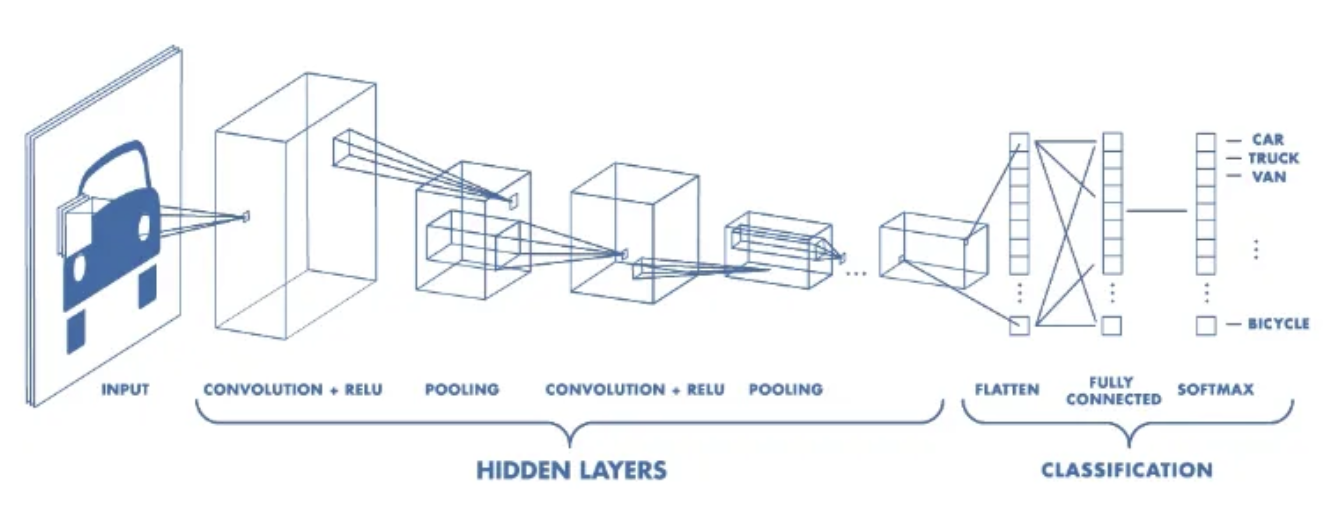
\includegraphics[width=0.9\textwidth]{images/conv2d2.png}
\caption{Structure of a 2D CNN. \cite{con2dart}}\label{fig:con2dart}
\end{figure}
In our first model we will implement six 2D Convolution Layers and three dense layers. With this we can expect an accuracy of $64\%$, however we aim to experiment with \acrshort{cnn} with a different amount of hidden layers and activation functions. In the convolution layers we have to set the following attributes: 
\begin{enumerate}
    \item Number of filters - This is the number of kernal, i.e. filters that a convolution layer will learn from. It is common that a convolution layer or network will learn many filters in parallel. This enables the network to recognize a greater amount of patterns in an image and is often refereed to as ``Computer vision''.
    \item Kernel size - The kernel is the neural network filter that moves across the image, scanning each pixel and converting the data into a smaller, or sometimes larger, format. It's good to use the kernel odd-sized kernel because of symmetry. We are interpolating the central pixel.
    \item Padding - Padding refers to the number of pixels added to an image when it is being processed by the kernel of a \acrshort{cnn}. Adding padding to an image processed by a \acrshort{cnn} allows for a more accurate analysis of images.
\end{enumerate}
We will implement a model with a similar structure as the model depicted in Figure \ref{fig:con2dart} and experiment with different parameters to try to achieve the best possible results. 

\begin{figure}[h]
\centering
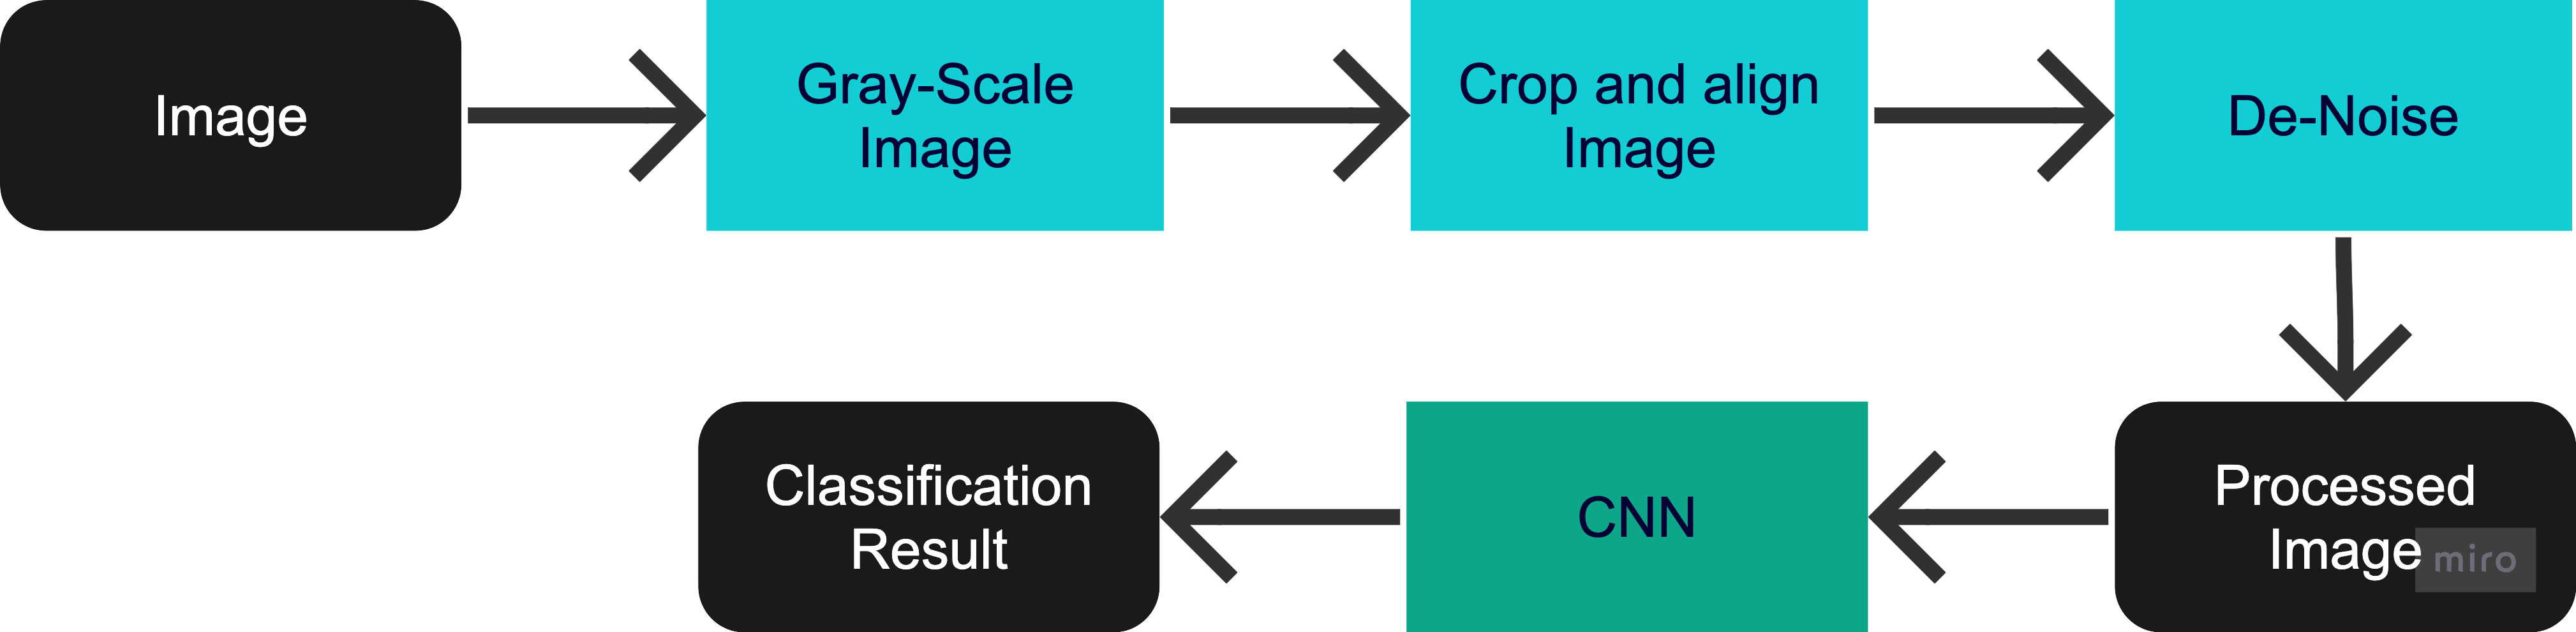
\includegraphics[width=0.9\textwidth]{images/fer-preprocessing-modelling.png}
\caption{Preprocessing and Modeling.}\label{fig:prep-mod}
\end{figure}
